\begin{frame}
    \begin{block}{Limites rencontrées}
        \begin{itemize}
            \item Propagation de l'épidémie uniforme
            \item Probabilité de contact humain uniforme
        \end{itemize}
    \end{block}

    \begin{center}
        \bf Les modèles stochastiques permettent de palier à ces limites.
    \end{center}
\end{frame}


\begin{frame}
    \frametitle{Reed et Forst}

    \begin{block}{Définition}
        L'infection mène d'abord à une période infectieuse, puis une période de rétablissement pour finir dans le groupe des immunisés. Les nouvelles infections se produisent par génération, séparées par la période de latence.
    \end{block}

    \begin{itemize}
        \item Le modèle est généralement utilisé avec une dynamique à temps discret, où la période infectieuse est courte et précédée d’une période de latence plus longue.
        \item Les probabilités dans chaque génération dépendent de l’état de l’épidémie dans la génération précédente, et sont spécifiées par des probabilités binomiales.
    \end{itemize}
\end{frame}

\begin{frame}
        \frametitle{Modèle SIR}

		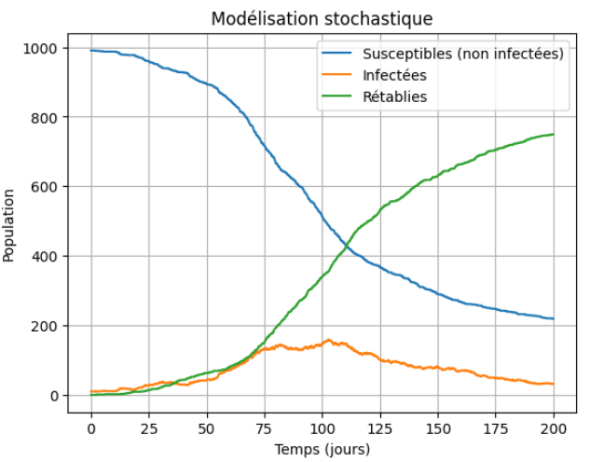
\includegraphics[width=0.45\linewidth, height=0.45\textheight, valign=c]{sir_stochastique}
		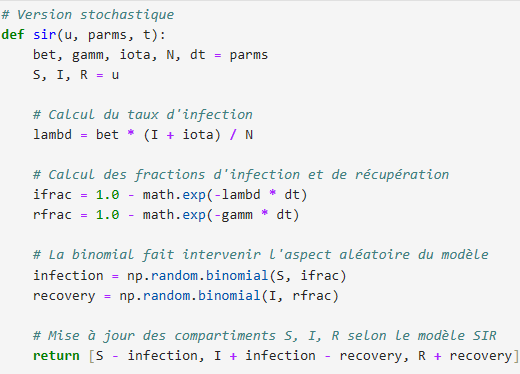
\includegraphics[width=0.5\linewidth, height=0.5\textheight, valign=c]{sir_stochastique_python_1}

        \begin{multicols}{2}
            \begin{itemize}
                    \item $\gamma = 0.05$
                    \item $\beta = 0.1$
                    \item $N = 1000$
                    \item $I_0 = 10$
            \end{itemize}
        \end{multicols}

\end{frame}

\begin{frame}
    \frametitle{Reed et Forst}

    \begin{alertblock}{Loi Binomiale}
        $$ P(X = k) = \binom{n}{k}p^k(1 - p)^{n-k} $$
    \end{alertblock}

    \begin{itemize}
        \item La loi Binomiale est la loi suivie par la variable aléatoire X qui compte le nombre de succès de n expériences de Bernoulli consécutives et indépendantes.
        \item La loi de Bernoulli est la loi suivie par l'expérience qui peut réussir avec une probabilité p.
    \end{itemize}
\end{frame}

\begin{frame}
    \frametitle{Reed et Forst}

    \begin{alertblock}{Définition}
        \begin{align}
            P &= P(Y_{j+1} = y_{j+1} | X_0 = x_0, Y_0 = y_0, ..., X_j = x_j, Y_j = y_j) \\
              &= P(Y_{j+1} = y_{j+1} | X_j = x_j, Y_j = y_j) \\
              &= \binom{x_j}{y_{j+1}}(1 - q^{y_j})^{y_{j+1}}(q^{y_j})^{x_j - y_{j+1}}
        \end{align}
    \end{alertblock}
\end{frame}
